%%%%%%%%%%%%%%%%%%%%%%%%%%%%%%%%%%%%%%%%%%%%%%%%%%%%%%%%%%%
% --------------------------------------------------------
% Tau
% LaTeX Template
% Version 2.4.4 (28/02/2025)
%
% Author: 
% Guillermo Jimenez (memo.notess1@gmail.com)
% 
% License:
% Creative Commons CC BY 4.0
% --------------------------------------------------------
%%%%%%%%%%%%%%%%%%%%%%%%%%%%%%%%%%%%%%%%%%%%%%%%%%%%%%%%%%%

\documentclass[9pt,a4paper,twocolumn,twoside]{tau-class/tau}
\usepackage[portuguese]{babel}
%% Spanish babel recomendation
% \usepackage[spanish,es-nodecimaldot,es-noindentfirst]{babel} 
%% Draft watermark
% \usepackage{draftwatermark}
%----------------------------------------------------------
% TITLE
%----------------------------------------------------------

\journalname{Relatório de Sistema de Controle 1 - Engenharia de Computação}
\title{Controle de Posição em Sistema Massa-Mola com Conexão Flexível}

%----------------------------------------------------------
% AUTHORS, AFFILIATIONS AND PROFESSOR
%----------------------------------------------------------

\author[a,1]{Rafael Anacleto Alves de Souza}
\author[a,2]{Elvis Correia Lopes dos Santos}
\author[a,3]{Guilherme de Oliveira Costa}
%\author[a,4]{Pedro de Carvalho Cedrim}


%----------------------------------------------------------

\affil[a]{Instituto de Computação, Universidade Federal de Alagoas – Campus A.C. Simões\\
\textsuperscript{1}\texttt{raas@ic.ufal.br}, 
\textsuperscript{2}\texttt{ecls@ic.ufal.br}, 
\textsuperscript{3}\texttt{goc@ic.ufal.br}}
%\textsuperscript{4}\texttt{pcc@ic.ufal.br}}

\professor{Prof. Dr. Icaro Bezerra Queiroz de Araujo}

%----------------------------------------------------------
% FOOTER INFORMATION
%----------------------------------------------------------

\institution{Instituto de Computação, Universidade Federal de Alagoas}
%\footinfo{Relatório elaborado com classe \LaTeX\ Tau}
\theday{setembro de 2025}
\leadauthor{Souza, Santos e Costa}
\course{Engenharia de Computação - Sistemas de Controle 1}

%----------------------------------------------------------
% ABSTRACT AND KEYWORDS
%----------------------------------------------------------

\begin{abstract}    
    O projeto tem como objetivo o estudo e implementação de um sistema de controle de posição em uma configuração massa-mola com duas massas acopladas por molas, representando situações práticas de sistemas com ligação elástica entre atuador e carga.
    O problema central consiste em manter a posição controlada da massa de saída, mesmo diante das oscilações e acoplamentos internos do sistema. Para isso, pretende-se desenvolver um modelo matemático e realizar simulações computacionais.
    O foco é a obtenção do modelo matemático que descreve a dinâmica do sistema e sua simulação em malha aberta, servindo de base para o projeto e implementação do controlador de posição.
\end{abstract}

%----------------------------------------------------------

\keywords{sistema massa-mola, controle de posição, acoplamento elástico, resposta dinâmica, two-mass system}

%----------------------------------------------------------

\begin{document}
		
    \maketitle 
    \thispagestyle{firststyle} 
    \tauabstract
    % \tableofcontents
    % \linenumbers 
    
%----------------------------------------------------------

\section{Introdução}

\taustart{O}objetivo deste trabalho é o desenvolvimento e análise de um modelo matemático para um sistema de controle de posição com acoplamento flexível. O protótipo, de configuração vertical, é composto por duas massas em cascata: a primeira massa ($M_1$) é suspensa por uma mola ($K_1$) e acoplada à segunda massa ($M_2$) por uma segunda mola ($K_2$). O controle de posição da massa inferior ($M_2$) será realizado por um servo motor que atua na parte uperior do sistema, sendo a posição monitorada por um sensor a laser.

Em sistemas industriais como braços robóticos e máquinas-ferramenta, a flexibilidade nos acoplamentos mecânicos introduz vibrações que degradam a precisão e podem levar à instabilidade. Portanto, a modelagem como um sistema de duas massas, em vez de uma massa única, é essencial para capturar essa dinâmica complexa e projetar controladores eficazes.

\section{Descrição do Sistema}

O sistema proposto neste projeto adota uma configuração vertical com duas massas acopladas, montadas em um arranjo em cascata. A primeira massa ($M_1$) é suspensa por uma mola ($K_1$). O ponto de suspensão desta mola é movimentado verticalmente por um sistema de engrenagem e correia, acionado por um servo motor (modelo DS3230MG). Esta primeira massa está acoplada à segunda massa ($M_2$) por uma mola de ligação ($K_2$), deixando $M_2$ suspensa. A rotação do motor atua no conjunto superior, provocando o deslocamento vertical de todo o sistema.

O objetivo do controle é a posição da massa inferior ($M_2$), que é medida continuamente por um sensor a laser posicionado na base da estrutura. 

Para evitar interferências mecânicas e vibrações laterais indesejadas, as massas são fixadas em carrinhos que deslizam ao longo de um trilho vertical. Esta configuração atua como um guia linear, restringindo o movimento transversal para garantir uma trajetória puramente vertical. O atrito gerado pelo deslizamento dos carrinhos no trilho é o principal componente do atrito viscoso ($b_1$ e $b_2$) considerado no modelo matemático.

A montagem do sistema foi pensada para minimizar problemas comuns em estruturas horizontais, como o atrito entre a base e os elementos móveis. A disposição vertical também facilita a análise do sistema em termos de energia potencial, amortecimento e resposta transitória sob a atuação da gravidade.

%figura 1 - modelo massa mola montado

\section{Revisão Bibliográfica}

O sistema massa-mola é um modelo físico fundamental para o estudo de fenômenos como vibrações, oscilações e ondas. Sua dinâmica é primariamente governada pela Lei de Hooke, que descreve a força restauradora da mola como sendo proporcional à sua deformação. Este modelo é amplamente aplicado na análise de sistemas do cotidiano, como suspensões de veículos e no projeto de estruturas como edifícios e pontes, para garantir sua estabilidade. Em sistemas físicos reais, apresença de forças dissipativas, como o atrito, introduz o fenômeno do amortecimento, que causa a redução da amplitude das oscilações ao longo do tempo. \cite{SistemaMassaMola}

Embora o modelo de massa única seja útil, ele se torna inadequado em diversas aplicações industriais, como máquinas-ferramentas, sistemas de manufatura de semicondutores, braçoes robóticos flexíveis e laminadores de aço. Nestes casos, atuadores e cargas são frequentemente conectados por acoplamentos flexíveis ou eixos longos de baixa rigidez. Essa flexibilidade introduz uma dinâmica mais complexa, que deve ser modelada como um sistema de duas ou  múltiplas massas. A elasticidade no acoplamento pode gerar vibrações que degradam significativamente a precisão do posicionamento e podem até levar à instabilidade do sistema de controle. Além disso, parâmetros como atrito e folgas mecânicas podem variar com o tempo e a temperatura, tornando o controle ainda mais desafiador. \cite{ComparativeStudy}

Para sistemas com orientação vertical, como o abordado neste projeto, a força da gravidade é uma consideração adicional. A literatura descreve duas abordagens para lidar com este efeito: a compensação ativa, que utiliza atuadores para gerar forças contrárias à gravidadem, e a compensação passiva, que utiliza elementos não energizados. A abordagem passiva é frequentemente preferida por ser mais simples, confiável, de menor custo e por não apresentar os problemas de instabilidade inerentes aos sistemas de controle ativo. Dentre os métodos passivos, destacam-se o uso de contrapesos e o de molas. Para aplicações que exigem baixa inércia e movimentos dinâmicos, os mecanismos baseados em molas são mais vantajosos, pois adicionam muito menos massa ao sistema. Uma técnica para projetar tais mecanismos é a abordagem energética, que busca manter a energia potencial total do sistema (gravitacional e elástica) constante para qualquer configuração. \cite{PassiveGravity}

Esta revisão da literatura, portanto, estabelece a relevância do presente trabalho. Fica evidente o desafio de controlar sistemas de duas massas devido às vibrações induzidas pela flexibilidade do acoplamento e a importância de considerar o efeito da gravidade em configurações verticais. A modelagem matemática e a análise de um sistema massa-mola de duas massas em arranjo vertical, considerando o atrito constituem o passo fundamental para o futuro projeto de controladores capazes de suprimir essas vibrações e garantir um controle de posição preciso, um problema de grande interesse na engenharia moderna. \cite{ComparativeStudy} \cite{PassiveGravity}

\section{Modelagem Matemática}

Nesta seção, a modelagem é desenvolvida a partir das Equações Diferenciais Ordinárias (EDO) que regem o sistema, considerando os efeitos do atrito. O sistema consiste em duas massas ($M_1$, $M_2$) acopladas por molas ($K_1$, $K_2$) e se movendo em um trilho que introduz atrito. O atrito viscoso do trilho e a resistência do ar são modelados como uma única força de amortecimento proporcional à velocidade, com coeficientes $b_1$ e $b_2$ para cada massa, respectivamente.

\subsection{Equações Diferenciais Ordinárias}

Aplicando a Segunda Lei de Newton para cada massa, definindo o deslocamento a partir da posição de equilíbrio, obtemos o seguinte sistema de EDOs:

Para a Massa 1 ($M_1$):

A força resultante em $M_1$ é a soma da força da mola $K_1$, da força da mola $K_2$, da força de atrito em $M_1$ e da força externa f(t).

\begin{equation}
    \sum F_{M_1} = -K_1 x_1(t) - b_1 \dot x_1(t) + K_2(x_2(t) - x_1(t)) + f(t) = M_1 \ddot{x}_1(t)
\label{eq:SomaM1}
\end{equation}

Reorganizando a equação, temos:

\begin{equation}
    M_1 \ddot{x}_1(t) + b_1 \dot x_1(t) + (K_1 + K_2) x_1(t) - K_2x_2(t) = f(t)
\label{eq:Reorg}
\end{equation}

Para a Massa 2 ($M_2$):

A força resultante em $M_2$ é a soma da força da mola $K_2$ e da força de atrito em $M_2$.

\begin{equation}
    \sum F_{M_2} = -K_2(x_2(t) - x_1(t)) - b_2\dot{x}_2(t) = M_2 \ddot{x}_2(t)
    \label{eq:M2}
\end{equation}

Reorganizando a equação, temos:

\begin{equation}
    M_2 \ddot{x}_2(t) + b_2\dot{x}_2(t) + K_2 x_2(t) - K_2 x_1(t) =  0
    \label{M2reorg}
\end{equation}

\subsection{Obtenção da Função de Transferência}

Para encontrar a função de transferência G(s) = $\frac{X_2(s)}{F(s)}$, aplicamos a Transformada de Laplace nas EDOs, assumindo condições iniciais nulas:

Para a EDO da Massa 1:

\begin{equation}
    (M_1s^2 + b_1s + K_1 + K_2)X_1(s) - K_2X_2(s) = F(s)
    \label{eq:EDOM1}
\end{equation}

Para a EDO da Massa 2:

\begin{equation}
    -K_2X_1(s) + (M_2s^2 + b_2s + K_2)X_2(s) = 0
    \label{eq:EDOM2}
\end{equation}

Da equação [\ref{eq:EDOM2}], podemos isolar $X_1$(s):

\begin{equation}
    X_1(s) = \frac{(M_2s^2 + b_2s + K_2)}{K_2}X_2(s)
    \label{eq:X1iso}
\end{equation}

Agora, substituimos está expressão para $X_1(s)$ na equação [\ref{eq:EDOM1}]:

\begin{equation}
    (M_1s^2 + b1s + K_1 + K_2)\left[\frac{(M_2s^2 + b_2s + K_2)}{K_2}X_2(s)\right] - K_2X_2(s) = F(s)
    \label{eq:substX1}
\end{equation}

Fatorando $X_2(s)$ e reorganizando os termos, encontramos a função de transferência final:

\begin{equation}
    G(s) = \frac{X_2 (s)}{F(s)} = \frac{K_2}{(M_1 s^2 + b_1 s + K_1 + K_2)(M_2 s^2 + b_2 s + K_2) - K_2 ^2}
\label{eq: FT}
\end{equation}

\begin{equation}
    G(s) = \frac{N(s)}{D(s)}
    \label{eq: FTresum}
\end{equation}

onde o numerador é $N(s) = \frac{K_2}{M_1M_2}$ e o denominador $D(s)$ é um polinômio de quarta ordem $D(s) = s^4 + a_3s^3 + a_2s^2 + a_1s + a_0$, cujos coeficientes são:
\begin{align}
    a_3 &= \frac{b_2}{M_2} + \frac{b_1}{M_1} \\
    a_2 &= \frac{K_2}{M_2} + \frac{K_1}{M_1} + \frac{b_1b_2K_2}{M_1^2M_2} \\
    a_1 &= \frac{b_1K_2 + K_1b_2 + K_2b_2}{M_1M_2} \\
    a_0 &= \frac{K_1K_2}{M_1M_2}
\end{align}

\begin{figure}[H]
    \centering
    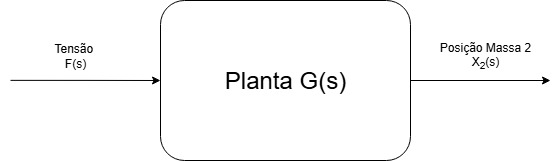
\includegraphics[width = 0.80\columnwidth]{DiagramaFT.jpg}
    \caption{Diagrama de blocos do sistema em malha aberta}
    \label{DiagramaFT}
\end{figure}

\subsection{Consideração sobre a Gravidade}

Para a configuração vertical, a força de gravidade ($F_G = M \cdot g$) atua constantemente em ambas as massas. Este efeito é responsável por estabelecer a posição de equilíbrio estático do sistema, ou seja, a gravidade estica as molas até um novo ponto de repouso. O modelo dinâmico e as EDOs foram desenvolvidas para deslocamentos ($x_1(t)$ e $x_2$(t)) a partir deste ponto de equilíbrio. Como a força da gravidade é constante, ela é cancelada pelas forças estáticas das molas no ponto de equilíbrio, e por isso o termo \textbf{g} não aparece na função de transferência dinâmica.

\begin{figure}[H]
    \centering
    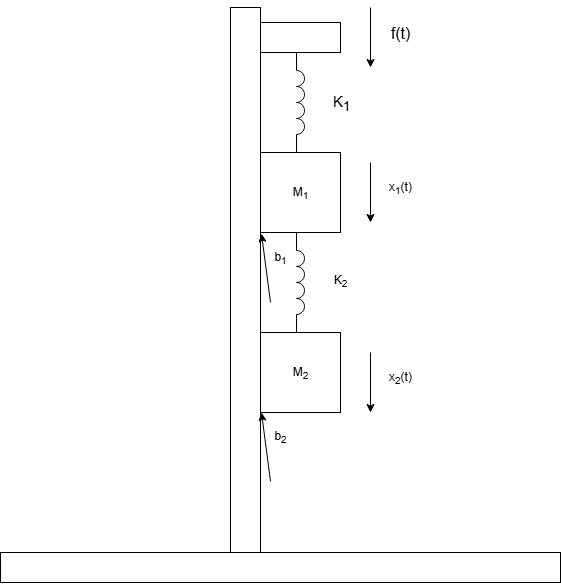
\includegraphics[width=0.80\columnwidth]{DiagramaForca.jpg}
    \caption{Modelagem do sistema massa-mola}
    \label{fig:MSM}
\end{figure}

%Criar um diagrama de blocos simples com uma entrada F(s), um bloco contendo G(s) e uma saída X2(s)

\section{Análise do Modelo}

\subsection{Característica da Função de Transferência}
A função de transferência G(s), apresentada na Equação \ref{eq: FTresum}, descreve as principais características dinâmicas do sistema. Primeiramente, observa-se que o modelo apresenta um sistema de quarta ordem, determinado pelo maior expoente da varíavel \textit{s} no polinômio do denominador, D(s).

Em relação à classificação, o sistema é de Tipo 0, pois não possui polos na origem (s = 0). Isso pode ser verificado pelo fato de o coeficiente de ordem zero do denominador, $a_0 = \frac{K_1K_2}{M_1M_2}$, ser diferente de zero para valores físicos não nulos dos parâmetros.

Outra característica fundamental é o Ganho Estático, que representa a resposta do sistema em regime estacionário a uma entrada constante. Ele é calculado fazendo $s = 0$ na função de transferência:

\begin{equation}
    G(0) = \frac{N(0)}{D(0)} = \frac{\frac{K_2}{M_1M_2}}{\frac{K_1K_2}{M_1M_2}} = \frac{K_2}{K_1K_2} = \frac{1}{K_1}
    \label{GE}
\end{equation}

Este resultado indica que, para uma força de entrada do tupo degrau unitário (1N), o deslocamento da Massa 2 em regime estacionário será de $\frac{1}{K_1}$ metros. Com o valor de $K_1 = 100 N/m$ utilizado na simulação, o ganho estático é $1/100 = 0.01$, o que confirma precisamente o valor de regime de $0.01 m$ observando no gráfico da resposta ao degrau \ref{fig:RDG}.

Finalmente, a função de transferência possui quatro polos e nenhum zero finito (pois numerador é uma constante). A localização exata dos polos depende dos parâmetros físicos, mas como discutido a seguir, a presença do atrito garante que eles estarão no semiplano esquerdo, resultando em um sistema estável.

\subsection{Análise de Estabilidade}

A estabilidade do sistema em malha aberta é determinada pelos polos da função de transferência, que são as raízes do polinômio característico do denominador:

\begin{equation}
    \Delta (s) = D(s) = s^4 + a_3s^3 + a_2s^2 + a_1s + a_0 = 0
\label{eq:raizes}
\end{equation}

Como o polinômio característico agora é um polinômio de quarta ordem completo, com termos de todas as potências de s. Consequentemente, para quaisquer valores físicos positivos dos parâmetros (M, b, K), os polos da função de transferência possuirão parte real negativa, deslocando-se do eixo imaginário para o semiplano esquerdo do plano s.

Isso garante que o sistema em malha aberta seja estável. O comportamento dinâmico esperado para uma entrada degrau é, portanto, uma resposta oscilatória amortecida, na qual o deslocamento da massa converge para um valor de regime estacionário após um período transitório. A localização exata dos polos e, por conseguinte, as características da resposta transitória -- como a frequência de oscilação amortecida e o tempo de acomodação -- dependem dos valores numéricos de todos os parâmetros físicos do sistema ($M_1, M_2, b_1, b_2, K_1, K_2$).

\section{Simulação Computacional}

Para validar o comportamento dinâmico previsto pelo modelo matemático, foi realizada uma simulação computacional utilizando o software MATLAB/Simulink.

Para a simulação, foram adotados valores preliminares para as constantes das molas, baseados em componentes comerciais comuns (ex: $K_1 = 100N/m$ e $K_2 = 150N/m$). É importante ressaltar que estes valores serão substituídos pelos valores reais medidos.

\begin{figure}[H]
    \centering
    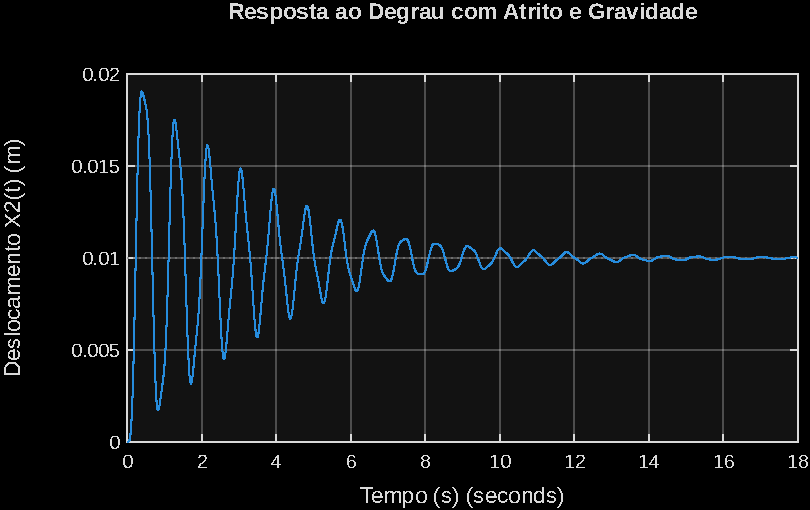
\includegraphics[width=0.75\columnwidth]{RespostaDegrauGravidade.pdf}
    \caption{Resposta ao Degrau}
    \label{fig:RDG}
\end{figure}

\begin{figure}[H]
    \centering
    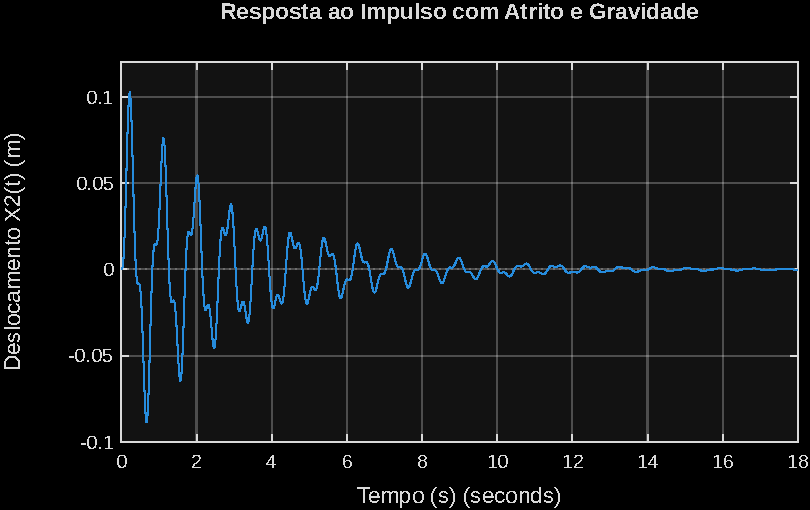
\includegraphics[width=0.75\columnwidth]{RespostaImpulsoGravidade.pdf}
    \caption{Resposta ao Impulso}
    \label{fig:RIG}
\end{figure}

%simulação do MATLAB, gerar gráfico da resposta ao degram e ao impulso e inseri-los

\subsection{Análise dos Resultados da Simulação}
Os resultados da simulação, apresentados nas Figuras \ref{fig:RDG} e \ref{fig:RIG}, confirmam visualmente a análise teórica do modelo desenvolvido. A resposta ao degrau (Figura \ref{fig:RDG}) exibe o comportamento característico de uma oscilação amortecida, onde o sistema, após um transitório oscilatório, converge para um valor de regime estacionário de aproximadamente 0.01 m. A presença de um sobressinal e a subsequente atenuação da amplitude das oscilações são consistentes com um sistema estável de ordem superior, como previsto.

De forma análoga, a resposta ao impulso (Figura \ref{fig:RIG}) mostra o sistema sendo deslocado de sua posição de equilíbrio e retornando a ela de forma oscilatória e amortecida, até cessar o movimento. A convergência em ambos os casos valida o caráter estável do sistema previsto pelo modelo que inclui os efeitos do atrito.

\section{Conclusão Parcial}

 A presente etapa do projeto culminou no desenvolvimento e simulação de um modelo matemático para o sistema de duas massas com acoplamento flexível. Foi obtida uma função de transferência que incorpora os parâmetros físicos do sistema, incluindo as massas, constantes elásticas e coeficientes de atrito, prevendo corretamente a natureza estável e de oscilação amortecida do sistema. A simulação computacional validou este comportamento dinâmico, fornecendo uma base sólida para a continuidade do projeto.

 O modelo agora verificado servirá como referência para a próxima etapa, que consistirá na montagem do protótipo físico e na sua validação experimental. O objetivo será determinar os parâmetros reais do sistema construído e comparar sua resposta a um sinal de entrada com os resultados simulados.



\printbibliography

%----------------------------------------------------------

\end{document}
